\section{Internal Block Diagram - MCS}
As with the Battery Management System, the Motor Control System (MCS) is too complex to be represented propely on a IBD along with the rest of the systems. The complexity has instead been visualized on a seperate Internal Block Diagram. The result is seen below.

\begin{figure}[H]
	\centering
	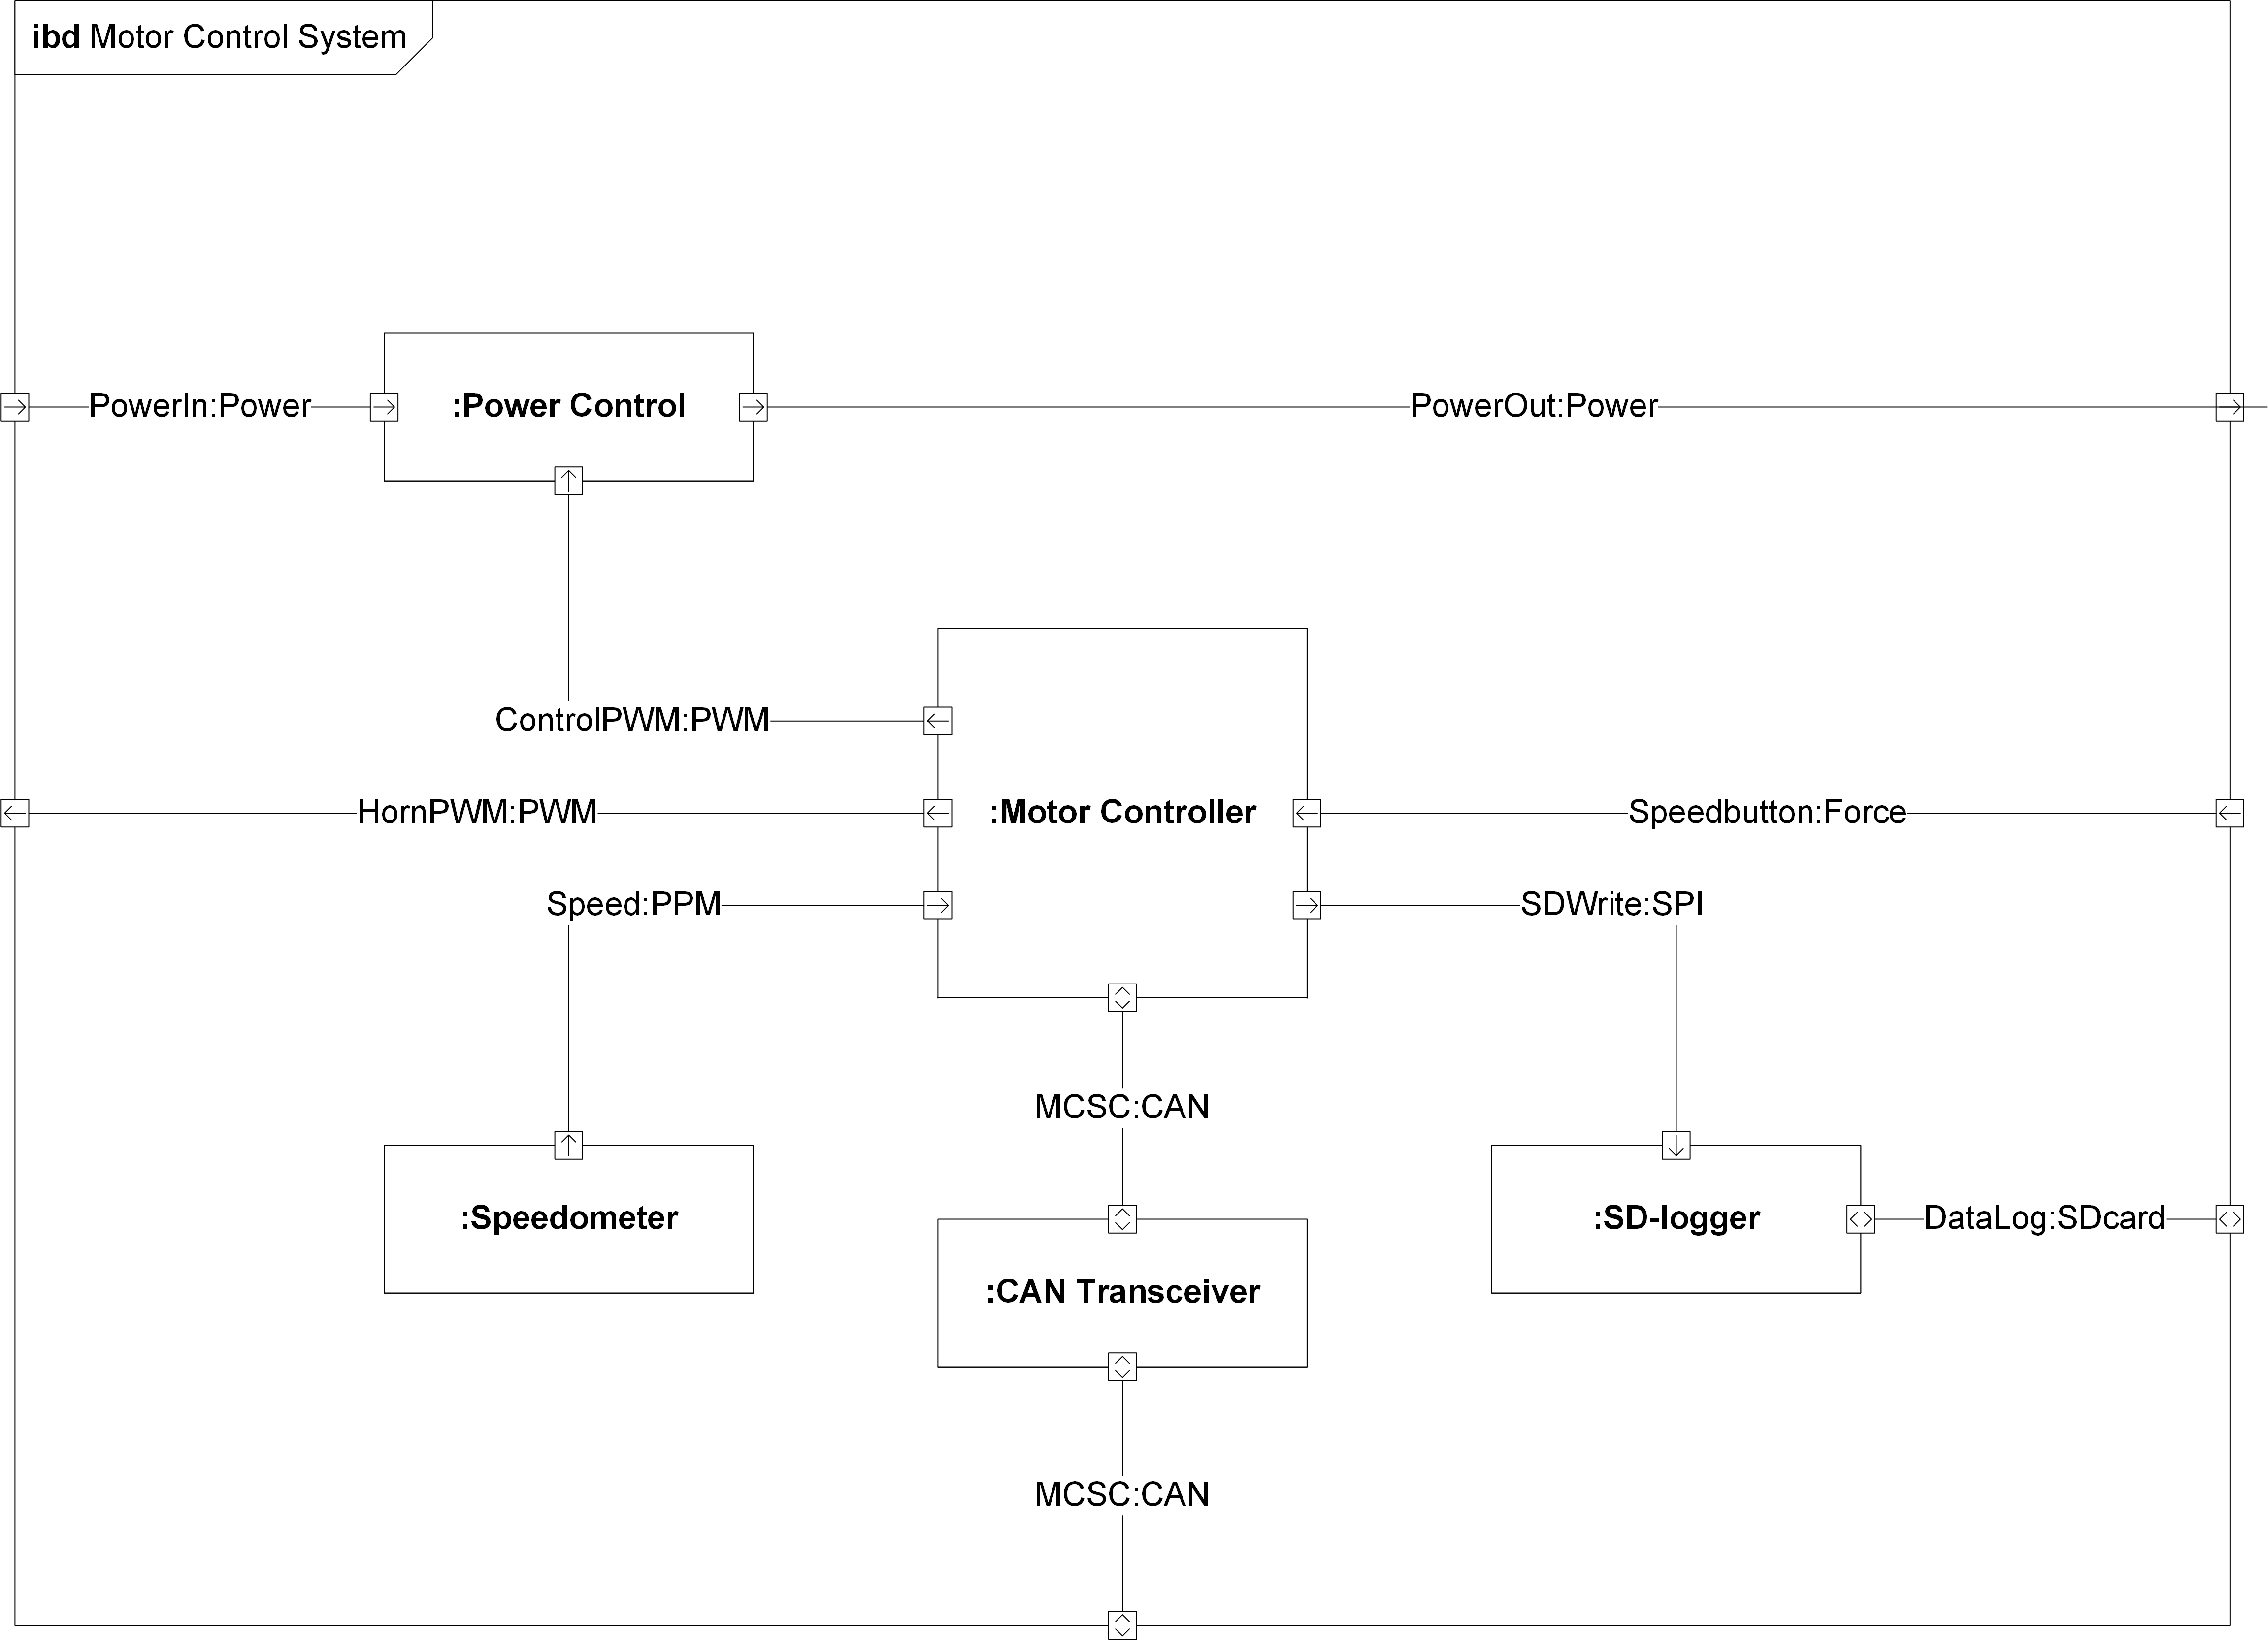
\includegraphics[width=1\linewidth]{Architecture/Diagrams/IBD_MCS}
	\caption{IBD for AU2's Motor Control System}
	\label{fig:IBD_MCS}
\end{figure}

It should be noted that each of the blocks in the MCS is connected with the signal called 'SupplyMCS:Voltage' which supplies every block in MCS with 5 V. This signal has been omitted from the IBD to increase the simplicity.

\section{Signal description - MCS}
The signals and protocols used to communicate between the blocks in MCS are specified in this section.

\textbf{Block :MCS}\\
Block interface description:
\begin{itemize}
	\item \textbf{SupplyMCS:Voltage}\\
	Direction: [External] $\rightarrow$ [Every Block]\\
	Description: Power supply to the systems.
	\item \textbf{HornPWM:PWM}\\
	Direction: [Motor Controller] $\rightarrow$ [External]\\
	Description: Sends out a square wave signal to supply the loudspeaker with an input.
	\item \textbf{PowerIn:Power}\\
	Direction: [External] $\rightarrow$ [Power Control]\\
	Description: Power coming from the batteries to supply the motor.
	\item \textbf{PowerOut:Power}\\
	Direction: [Power Control] $\rightarrow$ [External]\\
	Description: Power to supply the motor.
	\item \textbf{MCSC:CAN}\\
	Direction: [CAN Transceiver] $\rightarrow$ [External]\\
	Description: CAN connection to receive variables from BMS and to send to computer.
	\item \textbf{Speedbutton:Force}\\
	Direction: [External] $\rightarrow$ [Motor Controller]\\
	Description: Button to control the driving algorithm.
	\item \textbf{DataLog:SDcard}\\
	Direction: [SD-logger] $\leftrightarrow$ [External]\\
	Description: Button to control the driving algorithm.
\end{itemize}

\textbf{Block :Power Control}\\
Block interface description:
\begin{itemize}
	\item \textbf{SupplyMCS:Voltage}\\
	Direction: [External] $\rightarrow$ [Power Control]\\
	Description: Power supply to the block.
	\item \textbf{PowerIn:Power}\\
	Direction: [External] $\rightarrow$ [Power Control]\\
	Description: Power coming from the batteries to supply the motor.
	\item \textbf{ControlPWM:PWM}\\
	Direction: [Motor Controller] $\rightarrow$ [Power Control]\\
	Description: Signal from motor controller, decided by  coast and burn principle. 
	\item \textbf{PowerOut:Power}\\
	Direction: [Power Control] $\rightarrow$ [External]\\
	Description: Power to supply the motor.
\end{itemize}


\textbf{Block :Motor Controller}\\
Block interface description:
\begin{itemize}
	\item \textbf{SupplyMCS:Voltage}\\
	Direction: [External] $\rightarrow$ [Motor Controller]\\
	Description: Power supply to the block.
	\item \textbf{ControlPWM:PWM}\\
	Direction: [Motor controller] $\rightarrow$ [Power Control]\\
	Description: Signal from motor controller, decided by  coast and burn principle. 
	\item \textbf{HornPWM:PWM}\\
	Direction: [Motor controller] $\rightarrow$ [External]\\
	Description: Sends out a square wave signal to supply the loudspeaker with an input.
	\item \textbf{SDwrite:SPI}\\
	Direction: [Motor controller] $\rightarrow$ [SD-logger]\\
	Description: Information being written to SD card.
	\item \textbf{Speed:RPM}\\
	Direction: [Speedometer] $\rightarrow$ [Motor controller]\\
	Description: Square wave signal with a frequency corresponding to RPM.
	\item \textbf{Speedbutton:Force}\\
	Direction: [External] $\rightarrow$ [Motor controller]\\
	Description: Button to control the driving algorithm.
	\item \textbf{MCSC:CAN}\\
	Direction: [Motor Controller] $\leftrightarrow$ [CAN Tranceiver]\\
	Description: Tx/Rx signal to be converted to CAN or vice/versa.
\end{itemize}

\textbf{Block :Speedometer}\\
Block interface description:
\begin{itemize}
	\item \textbf{SupplyMCS:Voltage}\\
	Direction: [External] $\rightarrow$ [Speedometer]\\
	Description: Power supply to the block.
	\item \textbf{Speed:RPM}\\
	Direction: [Speedometer] $\rightarrow$ [Motor Controller]\\
	Description: Square wave signal with a frequency corresponding to RPM.
\end{itemize}

\textbf{Block :CAN Tranceiver}\\
Block interface description:
\begin{itemize}
	\item \textbf{SupplyMCS:Voltage}\\
	Direction: [External] $\rightarrow$ [CAN Tranceiver]\\
	Description: Power supply to the block.
	\item \textbf{MCSC:CAN}\\
	Direction: [Motor Controller] $\leftrightarrow$ [Can Tranceiver]\\
	Description: Tx/Rx signal to be converted to CAN or vice/versa.
	\item \textbf{MCSC:CAN}\\
	Direction: [Can Tranceiver] $\leftrightarrow$ [External]\\
	Description: CAN signal to be sent or received.
\end{itemize}

\textbf{Block :SD-logger}\\
Block interface description:
\begin{itemize}
	\item \textbf{SupplyMCS:Voltage}\\
	Direction: [External] $\rightarrow$ [SD-logger]\\
	Description: Power supply to the block.
	\item \textbf{SDWrite:SPI}\\
	Direction: [Motor controller] $\rightarrow$ [SD-logger]\\
	Description: Information being written to SD card.
	\item \textbf{DataLog:SDcard}\\
	Direction: [SD-logger ] $\leftrightarrow$ [External]\\
	Description: SD card can be disconnected from circuit in order to read information on PC.
\end{itemize}